\documentclass[12pt,fleqn]{article}\usepackage{../common}
\begin{document}
Ders 6

Ozvektor formulune tekrar bakalim

\[ Ay = \lambda y \]

Simdi tum ozvektorler ayni anda tek bir matris icinde olacak sekilde
ustteki formulun her ozvektor icin isleyecek ``kombine'' bir halini
yazabiliriz. $y_i$ vektorunun tum bir kolonu kaplayacak sekilde matrise
yazildigini dusunuyoruz. 

\[ 
A 
\left[\begin{array}{cccc}
\uparrow & \uparrow &  & \uparrow \\
y_1 & y_2 & ... & y_n \\
\downarrow & \downarrow &  & \downarrow 
\end{array}\right]
= 
\left[\begin{array}{cccc}
&&& \\
Ay_1 & Ay_2 & ... & Ay_n \\
&&& 
\end{array}\right]
\]

Buna gore ustteki esitligin sagindaki carpim da mantiklidir.Peki $Ay_i$
carpimi tanidik gelmiyor mu? Caprim ozvektor, ozdeger formulu. O zaman
$Ay_i = \lambda y_i$. Demek ki,

\[ 
\left[\begin{array}{cccc}
&&& \\
Ay_1 & Ay_2 & ... & Ay_n \\
&&& 
\end{array}\right]
= 
\left[\begin{array}{cccc}
&&& \\
\lambda_1y_1 & \lambda_2y_2 & ... & \lambda_ny_n \\
&&& 
\end{array}\right]
 \]

$\lambda$'lari disari cekebiliriz. 

\[ 
=
\left[\begin{array}{cccc}
&&& \\
y_1 & y_2 & ... & y_n \\
&&& 
\end{array}\right]
\left[\begin{array}{cccc}
\lambda_1 &&& \\
& .. && \\
&&& \lambda_n \\
\end{array}\right]
 \]

$\lambda$ matrisinde $\lambda$ olmayan yerler sifir degerini
tasiyor. Ozvektor matrisini $S$ olarak, caprazinda ozdegerleri tasiyan
matrisi $\Lambda$ olarak nitelersek

\[ AS = S\Lambda \]

Eger ustteki $S$ (ya da herhangi bir) matrisinin tum kolonlari birbirinden
bagimsiz ise $S$ tersine cevirelebilir (invertible) demektir. O zaman sunu
yapabiliriz:

\[ A = S \Lambda S^{-1} \]

Bu forma matrisin kosegenlestirilmesi (diagonalization) deniyor. 

Biraz zihin egzersizi: $A^2$ ne olur? 

\[ A^2 = (S \Lambda S^{-1})(S \Lambda S^{-1}) \]

\[ = S \Lambda S^{-1}S \Lambda S^{-1} \]

ortadaki $S$ ve $S^{-1}$ birbirini iptal eder. 

\[ = S \Lambda^2 S^{-1} \]

Bu bana ne soyluyor? $A^2$'nin ozvektorleri $A$ ile ayni, cunku formulun
$S$ ve $S^{-1}$ iceren kismi degismedi, ozdegerler ise $A$'nin
ozdegerlerinin karesi. Bu onceden buldugumuz $A^2y = \lambda^2y$ sonucu ile uyusuyor.

Peki, diyelim tersine cevirilebilir ise, $A^{-1}$ nedir? Ana formulden baslayalim

\[ A = S \Lambda S^{-1} \]

Tersine cevirme islemi esitligin sag tarafinda parantezin icinin sirasini
degistirir, sonra tersine cevirir, $S^{-1}$ ile baslariz, onun tersi $S$,
vs, ve sonuc

\[ A^{-1} = S \Lambda^{-1}S^{-1} \]

Ozvektorler matrislerinin yeri ve icerigi degismedi. Degisik olan tek sey
$\Lambda^{-1}$ ki bu matris icinde $1/\lambda_1$, $1/\lambda_2$, .. gibi
degerler olacak. Diger bir acidan kontrol edelim:

\[ Ay = \lambda y \]

\[ y = \lambda A^{-1} y \]

\[ \frac{1}{\lambda}y =  A^{-1} y \]

Bu ustteki sonuc ile ayni seyi soyluyor. $A^{-1}$'in tersi ayni $y$
ozvektor(ler)e sahip, ve solda olan ozdeger oncekine kiyasla $1/\lambda$
degerinde. 

Tabii tum bunlara baslamadan once ``$\lambda$'nin sifir olmadigi
durumlarda'' demeliydim, cunku bu sifirlik durum bize $A$'nin tersine
cevirilir olmadigi yonunde bir isaret olurdu. Terminoloji olarak bir tane
bile sifir ozdeger $A$ tekilsel (singular) demektir, eger hicbiri sifir
degilse $A$ tersine cevirilebilir demektir. 

Bir simetrik $K$ matrisini ele alalim, simetrik oldugu icin tum ozdegerleri
reel sayilar, ve ozvektorleri birbirine dik (orthagonal). 

Dik yerine normalize edilmis (normalized) da diyebilirdik, numerik paketler
(Python gibi) cogunlukla birimsellestirilmis, yani uzunlugu 1 olan
vektorler dondurur, ve ozdeger/vektor ikilisi icin zaten yon onemlidir, hem
ozdeger hem ozvektoru 2 ile carpip ayni seyi elde edebiliriz mesela.

Uzunluktan bahsederken, onu daha once $y_i^T \cdot y_j$ olarak gosterdik,
ki simetrik bir matrisin dik ozdegerleri icin bu $y_i^T \cdot y_j = 0, \ i
\ne j$. 
Normalize edilmis bir ozvektorun kendisi ile noktasal carpimi nedir? 
$y_i^T \cdot y_i = 1$ cunku vektor birimsel, uzunlugu 1. Tum
ozdegerleri iceren matris uzerinden bu hesabi yapabilir miyiz? Daha once
yarattigimiz su matris ile baslayalim:

\[ 
\left[\begin{array}{cccc}
\uparrow & \uparrow &  & \uparrow \\
y_1 & y_2 & ... & y_n \\
\downarrow & \downarrow &  & \downarrow 
\end{array}\right]
\]

sol tarafina devrigini (transpose) koyalim

\[ 
\left[\begin{array}{ccc}
\leftarrow & y_1^T & \rightarrow \\
 & ... & \\
\leftarrow & y_n^T & \rightarrow 
\end{array}\right]
\left[\begin{array}{cccc}
\uparrow & \uparrow &  & \uparrow \\
y_1 & y_2 & ... & y_n \\
\downarrow & \downarrow &  & \downarrow 
\end{array}\right]
\]

Bu carpimi yaparsak sonuc ne olacak? Mesela $y_1^T$ ile $y_1$ carpimi 1
degerinde, $y_1^T$ ile diger her carpim sifir. Boyle gider. Ve sonuc olarak
caprazinda 1 diger her yerinde 0 iceren birim (identity) matrisini elde
ederiz.

Uzerine basarak soyleyelim, bu simetrik matrisler icin, cunku diger $A$
matrisleri icin ozvektorlerin hepsinin birbirine dik olmasini
bekleyemeyiz. 

Devam edelim, o zaman ustteki hesabi kisaca gosterirsek

\[ S^T S = I \]

Bu hakikaten cok onemli bir sonuc. 

Usttekinin dogru oldugu durumlarda $S$ harfini degistirirsek aslinda daha iyi
olur boylece ozvektor matrisinin bir simetrik $K$ matrisinden geldigini
daha iyi goruruz. Bu durumlarda $Q$ harfini kullanalim. 

$Q$'ye bir ``dik matris'' te denebilir, cunku $Q^TQ = I$. Bu ifadeye
bakarak baska bir sey daha soyleyebiliriz, $Q$'yu baska \textbf{ne} soldan
carparsa sonuc birim matristir? $Q^{-1}$. O zaman $Q^T = Q^{-1}$ de
diyebiliriz.

Bir dik matris ornegi gorelim:

\[ 
\left[\begin{array}{cc}
\cos \theta & -\sin \theta \\
\sin \theta & \cos \theta \\
\end{array}\right]
 \]

Ilk kolona bakalim, uzunlugu hakikaten 1, cunku $\cos \theta ^2 + \sin \theta
^2 = 1$. 
Diger kolon da ona dik, 1. kolon ile carpilinca sonuc sifir olacak. 

Not: Ustteki matrise ``$\theta$ kadar donduren matris'' ismi de verilir,
eldeki bir $v$ vektorunu $Q$ ile carpimi, yani $Qv$, o vektoru uzunlugunu
degistirmeden $\theta$ kadar dondurecektir.

Devam edelim

\[ K = S \Lambda S^{-1} \]

$S$ yerine $Q$ kullanmaya karar vermistik

\[  K = Q \Lambda Q^{-1} \]

O zaman, daha onceden gordugumuz esitlik uzerinden, 

\[  K = Q \Lambda Q^{T} \]

Su guzellige bakin. Buna mekanikte ana eksen teoremi (principal axis
theorem), matematikte spektral teoremi (spectral theorem), kuantum
mekanikte caprazlastirma (diagonalization) ismi verilir, her yerde ortaya
cikar, pek cok sekilde kullanilir. Ne zaman elde bir simetrik matris var
ise, o zaman ustteki tanim kullanilabilir demektir.

$K$ matrisine geri donelim. 

\[ 
K =
\left[\begin{array}{rrrrr}
2 & -1 &&& \\
-1 & \ddots & \ddots && \\
& \ddots &&& \\
&&&& \\
&&&& 
\end{array}\right]
 \]

Bu matris ikinci farkliliklari ayriksal olarak temsil etmek icin
kullanilmisti, esnek cubugu temsil ettigi zaman sabit / sabit problemini
cozuyordu. $K$ surekli (continuous) baglamda hangi diferansiyel
denklemi temsil edecektir? $-d^2y/dx^2$.  Ozdeger, ozvektor olarak ise

\[ Ky = \lambda y \]

Soyle bir gecis yapilabilir

\[ -\frac{d^2y}{dx^2} = \lambda y(x) \]

Burada ilginc bir numara var: daha once surekli fonksiyondan basliyorduk,
sonra $K$ matrisi uzerinden ayriksal hale geciriyorduk. Hoca burada
ozdeger, ozvektor formundan basladi, ve surekli forma gecti. Sonra ustteki
denklemin cozumunu bulunca, tekrar geri gidecek, ve ayriksal olarak
ozvektorlerin birbirine dikligini gorecegiz, ve bunun surekli baglamda da
hala gecerli oldugunu anlayacagiz. 

Cozumu bulmak icin tahmin yontemini kullanalim: hangi fonksiyonun ikinci
turevinin negatifi, o fonksiyonun katini verir? Sin ve cos fonksiyonlari,
yani $y$ $\sin \omega x$, $\cos \omega x$ olabilir, ya da onlarin birlesimi
olarak ustel $e^{-i\omega x}$, $e^{i\omega x}$ formunda olabilir.

Eger $y$ icin $\sin, \cos$ kullanirsak ozdeger ne olur? Yerine koyarsak
goruruz, $\sin\omega x$'in iki kere turevini alirsak $\omega$ iki kere
disari cikar, arada bir eksi degeri mutlaka ortaya cikar (cunku 
$\cos'\theta = -\sin\theta)$, eksi ile eksi carpilir, sonuc $\omega^2$. 
Hatta ustteki tum $y$ secenekleri icin sonuc aynidir. 
 
Sinir kosullarini unutmayalim tabii. Problemin tamami

\[ -\frac{d^2y}{dx^2} = \lambda y(x) \]

\[ y(0) = 0, \ y(1) = 0 \]

Sinir kosullari sayesinde tum $\sin$, tum $\cos$ fonksiyonlari arasindan belli
bazilarini secebilecegiz. En basit eleme $y(0) = 0$, bu sart sayesinde cos
fonksiyonlarinin tamami elenir. Degil mi? Cunku $\cos(0) = 0$ dogru
olamaz. Diger sarta bakalim, $y(1)$ uzerinden $\sin(\omega) = 0$ olur,
tersinden dusunursek $\sin(\omega)$ ile sifir degeri verecek $\omega$ ne
olabilir? $\pi$ olabilir. O zaman bir cozum bulduk:

\[ y_1 = \sin \pi x \]

Elimizdeki ilk ``ozfonksiyon (eigenfunction)'' bu. Ozdegeri nedir?

\[ \lambda_1 = \pi^2 \]

cunku ustte belirttik, $\omega^2$, o zaman $\pi^2$. 

Ikinci deger ne olur? $2\pi$. 

\[ y_2 = sin2\pi x, \ \lambda_2 = (2\pi)^2 = 4\pi^2 \]

Eger sinir sartlarini degistirseydim, serbest / serbest, serbest / sabit
gibi, o zaman farkli $y$ degerleri elde ederdim. Mesela ilk sinir sarti
$y'(0) = 0$ olsaydi, sin fonksiyonlari yerine cos fonksiyonlari elde
ederdik, sin elenirdi cunku sin'in turevi $\cos(0) = 0$ dogru bir ifade
olamazdi. 

Ayriksal olarak temsil edersek, $\sin\pi h$ ve $h = 1 / n+1$, $n = 4$
kullanalim

\[ 
y_1 = 
\left[\begin{array}{c}
\sin \frac{\pi}{5} \\
\sin \frac{2\pi}{5} \\
\sin \frac{3\pi}{5} \\
\sin \frac{4\pi}{5} 
\end{array}\right]
 \]


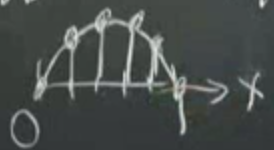
\includegraphics[height=2cm]{6_2.png}

Bu da ikinci ozvektor (ozfonksiyon). 

\[ 
y_2 = 
\left[\begin{array}{c}
sin \frac{2\pi}{5} \\
sin \frac{4\pi}{5} \\
sin \frac{6\pi}{5} \\
sin \frac{8\pi}{5} 
\end{array}\right]
 \]

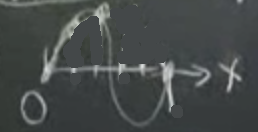
\includegraphics[height=2cm]{6_3.png}

Ozvektorler oldugunu soylemekle ikinci bir sey daha soyluyoruz, bu iki
vektor birbirine dik. Buradan hareketle $\sin(\pi x)$ fonksiyonu (iki
ustteki resim) $\sin(2\pi x)$ fonksiyonuna (bir ustteki resim) dik
diyebilirdik, ki hakikaten oyledir. Hatta bu matematiksel durum Fourier
Serilerinin islemesini saglayan onemli bir etkendir.

Bu baglantidan devam edelim: pur vektorler oldugu zaman diklik kontrolu icin
$y_1^T \cdot y_2$ diyordum, ve $y_1$ ve $y_2$'nin eslesen elemanlari birbiriyle 
carpilip, bu sonuclar teker teker toplaniyordu. Elimde $y_1$ ve $y_2$ icin 
birer fonksiyon var ise, bir tarafta $\sin(\pi x)$ var, her $x$ icin degisik
degerler veriyor, diger tarafta $\sin(2\pi x)$ var, bunlari carpip toplamam
lazim. Ama Elimde teker teker toplayabilecegim degerler olmadigi icin ($x$ reel
bir sayidir, belli bir aralikta bile sonsuz tane degere sahip olabilir), o
zaman toplama yerine entegrasyon kullanmam lazim. O zaman

\[ y_1^T \cdot y_2  = \int_0^1 (\sin \pi x)(\sin 2\pi x)dx  \]

Sonuc sifir gelecek, cunku iki fonksiyon birbirine dik.

Soru 1.5.3

\begin{minted}{python}
import scipy.linalg as lin

def ktbc(n):
    vec = np.zeros((1,n))
    vec[0,0] = 2
    vec[0,1] = -1
    K = lin.toeplitz(vec)
    T = np.copy(K)
    T[0,0] = 1
    B = np.copy(K)
    B[0,0] = 1
    B[n-1,n-1] = 1
    C = np.copy(K)
    C[n-1,n-1] = 1
    
    return K, T, B, C

import scipy.linalg as lin
import ktbc

K,T,B,C =  ktbc.ktbc(5)

u,v=lin.eig(K)

print u

print 2-np.sqrt(3), 2-1, 2-0, 2+1, 2+np.sqrt(3)

print 2*np.ones((5,1)).T - 2*np.cos((np.arange(5)+1) * np.pi/6)
\end{minted}

\begin{verbatim}
[ 3.73205081+0.j  3.00000000+0.j  2.00000000+0.j  0.26794919+0.j
  1.00000000+0.j]
0.267949192431 1 2 3 3.73205080757
[[ 0.26794919  1.          2.          3.          3.73205081]]
\end{verbatim}


\end{document}

